\documentclass[12pt, a4paper]{article}
\usepackage[utf8]{inputenc}
\usepackage[T2A]{fontenc}
\usepackage[russian]{babel}
\usepackage[oglav,spisok,boldsect,eqwhole,figwhole,hyperref,hyperprint,remarks,greekit]{fn2kursstyle}



\usepackage{subfig}
%\usepackage{amsmath}
%\usepackage{amssymb} 
\usepackage{amsfonts}
\usepackage{mathtools}
\usepackage{enumitem}
\usepackage{pifont}
\usepackage{changepage}
\usepackage{multirow}
\usepackage{supertabular}
\usepackage{multicol}

\graphicspath{
	{./style/}
	{../wolfram/f_22600_10.08.26/plots/}
	{../wolfram/f_22601_10.08.26/plots/}
	{../wolfram/f_22609_10.08.25/plots/}
	{../wolfram/f_22608_10.08.28/plots/}
	{./illustr/}
}

%\usepackage{multirow}
%\usepackage{supertabular}
%\usepackage{multicol}

\frenchspacing
\sloppy
\counterwithout{equation}{section}
\counterwithout{figure}{section}
\newenvironment{comment}{}{}




% Параметры титульного листа
\title{Поиск потенциала электрического поля в периодической структуре}
\author{А.\,Д.~Егоров}
\supervisor{К.\,Е.~Казаков}
\group{ФН2-62Б}
\date{2023}

% Переопределение команды \vec, чтобы векторы печатались полужирным курсивом
\renewcommand{\vec}[1]{\text{\mathversion{bold}${#1}$}}%{\bi{#1}}
\renewcommand{\phi}{\varphi}

\newcommand\thh[1]{\text{\mathversion{bold}${#1}$}}
%Переопределение команды нумерации перечней: точки заменяются на скобки
%\renewcommand{\labelenumi}{\theenumi)}
\renewcommand{\labelenumii}{\arabic{enumi}.\arabic{enumii}}
\renewcommand{\labelenumiii}{\arabic{enumi}.\arabic{enumii}.\arabic{enumiii}}
\renewcommand{\labelenumiv}{\arabic{enumi}.\arabic{enumii}.\arabic{enumiii}.\arabic{enumiv}}


\begin{document}
	
	\maketitle	
	\tableofcontents
	\newpage
	
	\section-{Введение}
		
	
	\section {Постановка задачи}
		
		Найти потенциал электрического поля между двумя бесконечными пластинами, профиль одной из которых плоский, а профиль другой описывается некоторой периодической функцией. Значения потенциала на пластинах заданы и константны.		
		
		
	%\newpage
	\section{Обзор задачи}
		\looser{-0.02}{Для постоянного электрического (электростатического) поля уравнения Максвелла имеют вид}
		\begin{equation}
			\mathrm{div} \vec{\mathrm{E}} = 4 \pi \rho,
			\label{div_E}
		\end{equation}
		\begin{equation}
			\mathrm{rot} \vec{\mathrm{E}} = 0,
			\label{rot_E}
		\end{equation}
		где $\rho$ --- объемная плотность внешних зарядов. Электрическое поле $\vec{\mathrm{E}}$ выражается через только скалярный потенциал соотношением
		\begin{equation}
			\vec{\mathrm{E}} = -\mathrm{grad} \varphi,
			\label{E_grad_phi}
		\end{equation}
		подставляя (\refeq{E_grad_phi}) в (\refeq{div_E}), получим уравнение, которому удовлетворяет потенциал постоянного электрического поля:
		\begin{equation}
			\Delta \varphi = - 4 \pi \rho.
			\label{Pois_eq}
		\end{equation}
		Уравнение (\refeq{Pois_eq}) есть уравнение Пуассона. При $\rho = 0$, т.е. при отсутствии внешних сил, потенциал удовлетворяет уравнению Лапласа
		\begin{equation}
			\Delta \phi = 0.
			\label{Laplace_eq}
		\end{equation}
		
		\subsection{Математическая постановка задачи}
			
			Из условия поставленной задачи известно, что внешних сил нет, следовательно, потенциал электростатического поля должен удовлетворять уравнению (\refeq{Laplace_eq}). Через функцию $w(x)$ зададим профиль искривленной пластины, $w(x)$  --- некоторая периодическая функция с периодом $T$, т.е. $w(x) = w(x + T)$. Пусть плоская пластина находится над искривленной на уровне $y_a$. Значение потенциала на пластинах заданы и константны, обозначим значение на верхней (плоской) пластине как $\phi_a$, на нижней (искривленной) --- $\phi_w$. Т.к. профиль профиль задан периодической функцией, следовательно необходимо использовать условие равенства потенциалов в точках $x$ и $x + T$, т.е. $\phi (x, y) = \phi (x + T, y)$.
			
			Из этих условий составим систему, которую требуется решить: 		
			\begin{equation}
				\begin{cases}
					\Delta \phi (x, y)  = 0, \\
					\phi (x, y_a) = \phi_a, \\
					\phi (x, w(x)) = \phi_w, \\
					\phi (x, y) = \phi (x + T, y),\\
					
				\end{cases}
			\end{equation}
			\begin{figure*}[!h]
				\centering
				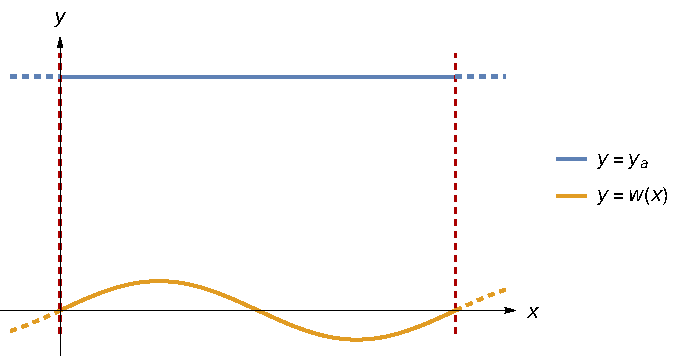
\includegraphics[width=0.65\textwidth]{illustr.pdf}
				\caption{Иллюстрация области, в которой будет решаться задача}
				\label{fig:f_22608_100828_mod_opt_knot_comparison}
			\end{figure*}
			

	\newpage
	\section{Программная реализация алгоритма}
		
		Построение сеток --- Wolfram Mathematica, алгоритм метода конечных элементов реализован на языке C++
	
	\section-{Заключение}
	
	
	\newpage
	
	\begin{thebibliography}{4}
		
		
		\bibitem{python} Python.  A high-level, general-purpose programming language \\
		URL:  \href{https://www.python.org/}{https://www.python.org/} \\
		(дата обращения 20.10.2022)
		
		\bibitem{jupyter} Project Jupyter. Web-based interactive development environment \\
		URL:  \href{https://jupyter.org/}{https://jupyter.org/} \\
		(дата обращения 20.10.2022)
		
		\bibitem{numpy} NumPy. The fundamental package for scientific computing with Python\\
		URL:  \href{https://numpy.org/}{https://numpy.org/} \\
		(дата обращения 5.01.2023)
		
		\bibitem{scipy} SciPy. Fundamental algorithms for scientific computing in Python \\
		URL:  \href{https://scipy.org/}{https://scipy.org/} \\
		(дата обращения 6.01.2023)
		
		
		
		
		
		
		
		
		
	\end{thebibliography}
	

\end{document}